\section{\textcolor[rgb]{1.00,0.00,0.00}{User study}}
\label{sec:user_study}
\textcolor[rgb]{1.00,0.00,0.00}{ To investigate the user experience of \sysname, we also conduct an usability evaluation on the 112 participants in Section~\ref{sec:eval}.  The aim of this part is to demonstrate that \sysname is operable in practice and can guide the user for blood glucose control. The target users includes both non-diabetes individuals and type I and type II diabetic patients, which are two main types of diabetes mellitus \cite{bib:Diabetes_mellitus}. \sysname monitors the blood glucose every 3 minutes, which is a fine-grained interval to track the blood glucose dynamics. When it detects an abnormal blood glucose event, the user will be reminded to take corresponding treatment (\eg, double-check by finger pricking or using CGM devices).
Note that \sysname is not an alternative of CGMs or the finger sticker, but is a supplement while it is inconvenient for users to take clinic measurement. For example, assuming an user measuring blood glucose by finger-stick at 9 a.m. and 8 p.m., he can wear \sysname to monitor his blood glucose dynamic in other time.  The blood glucose data predicted by \sysname helps users ameliorate their daily activities ( \eg food intakes and exercise), and also assists doctors to make more efficient and comprehensive treatment on patients.}

\subsection{Procedure}
We designed a semi-structured questionnaire to collect the qualitative and quantitative feedbacks from 112 participants about their usage of \sysname. The contents of questionnaire are mainly about two aspects of \sysname: 1) the usability of system in daily life and 2) the instructions to blood glucose control.
Since most of the participants are not proficient in English, the questionnaire was written as their native language, and we translated their response to English as consistently as possible for the report in this paper.
All the participants were asked to answer the questions seriously and were compensated about \$20 in a local currency at the end of this study.

\subsection{Results}

\subsubsection{The usability of \sysname}
\sysname provides the scroll menus as the application program interfaces on the selections of food, drug and insulin injection (as shown in Fig.\ref{fig:usibility_UI}). A camera button is also provided for users to take pictures of their food, which can be extended to recognize food items automatically by computer vision techniques \cite{bib:yang2010food, bib:kawano2013real}.
Moreover, the users can also set specific time points on \sysname for recording reminders.

\begin{figure}[h]
  \centering
  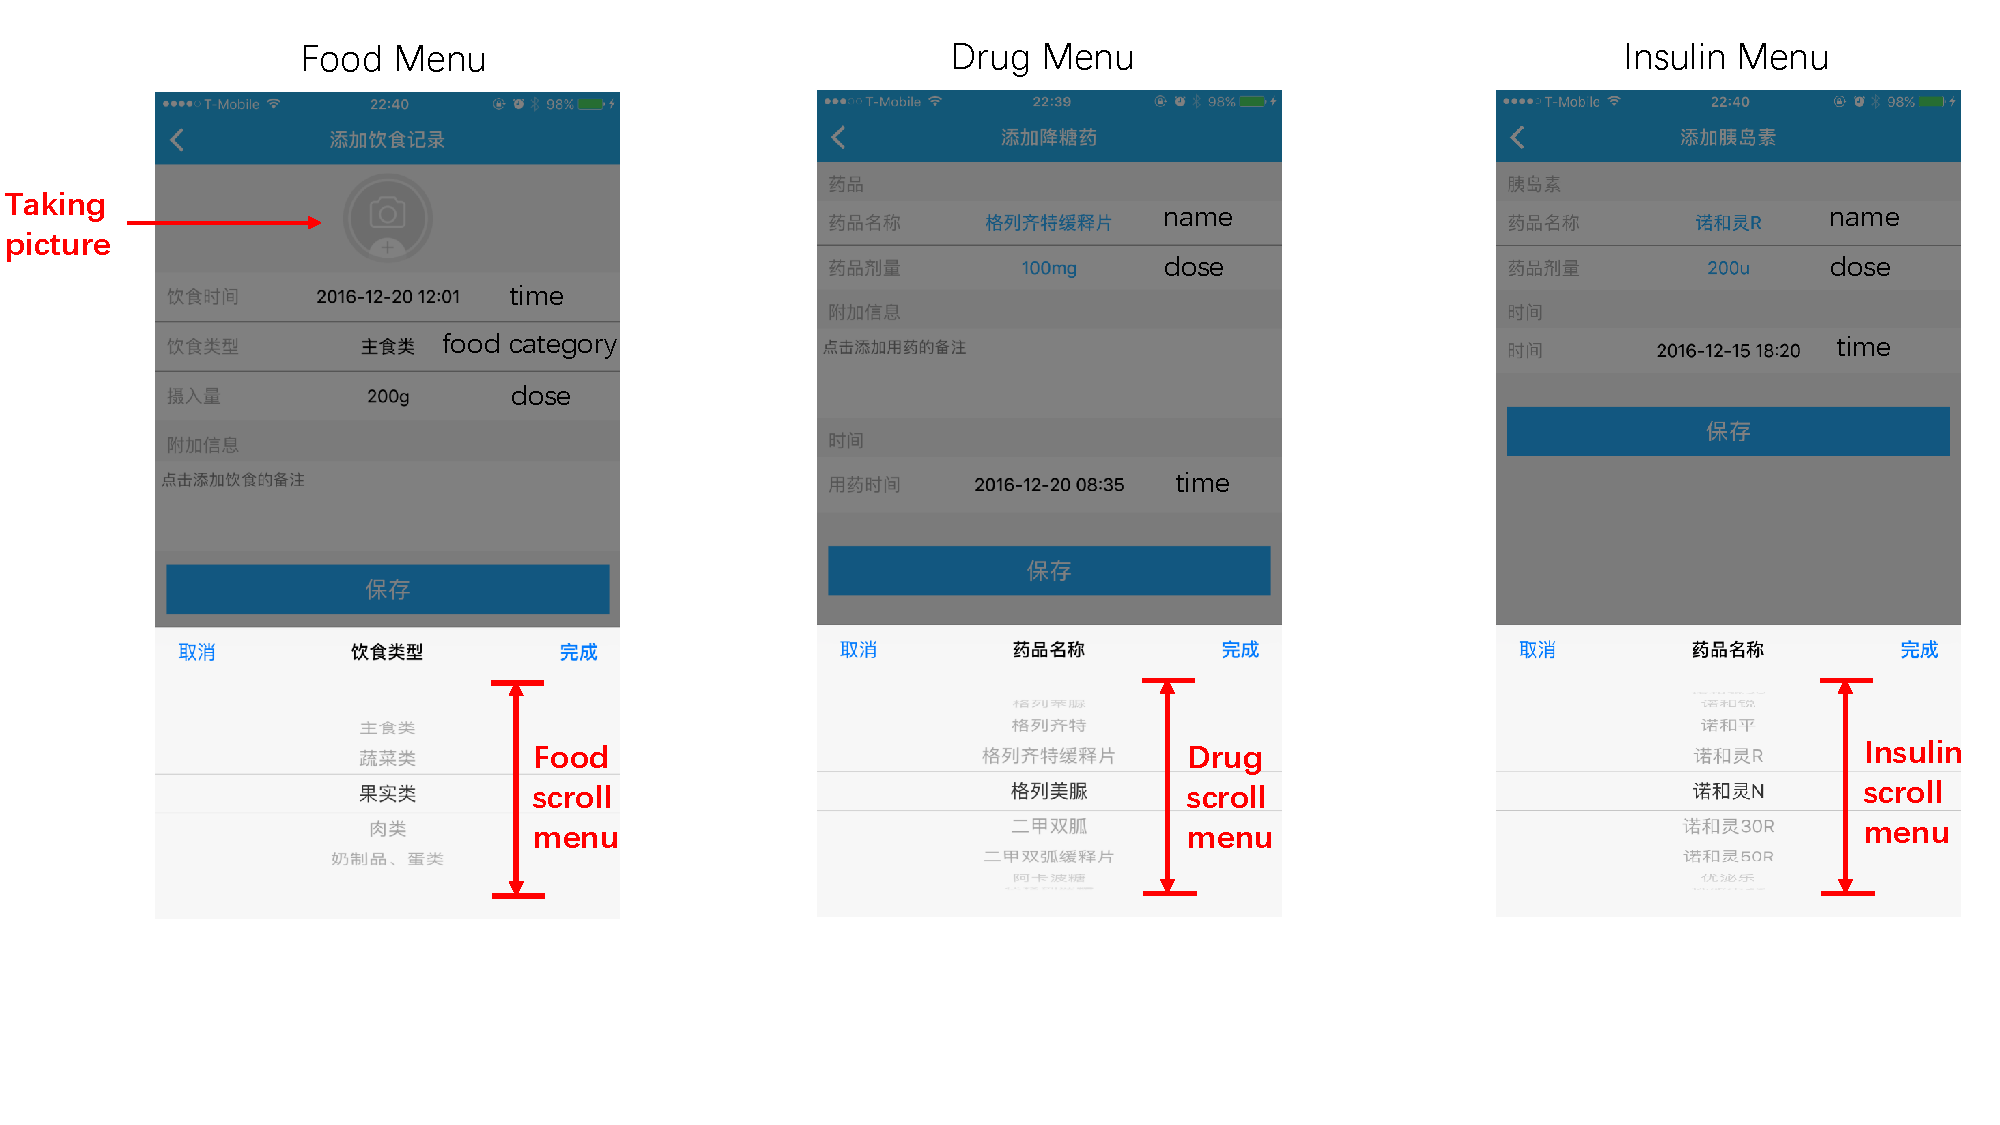
\includegraphics[width=0.9\columnwidth]{./img/usibility_UI.pdf}
  \caption{User interfaces of food, drug and insulin recording menus}
  \label{fig:usibility_UI}
\end{figure}

\begin{figure}[h]
  \centering
  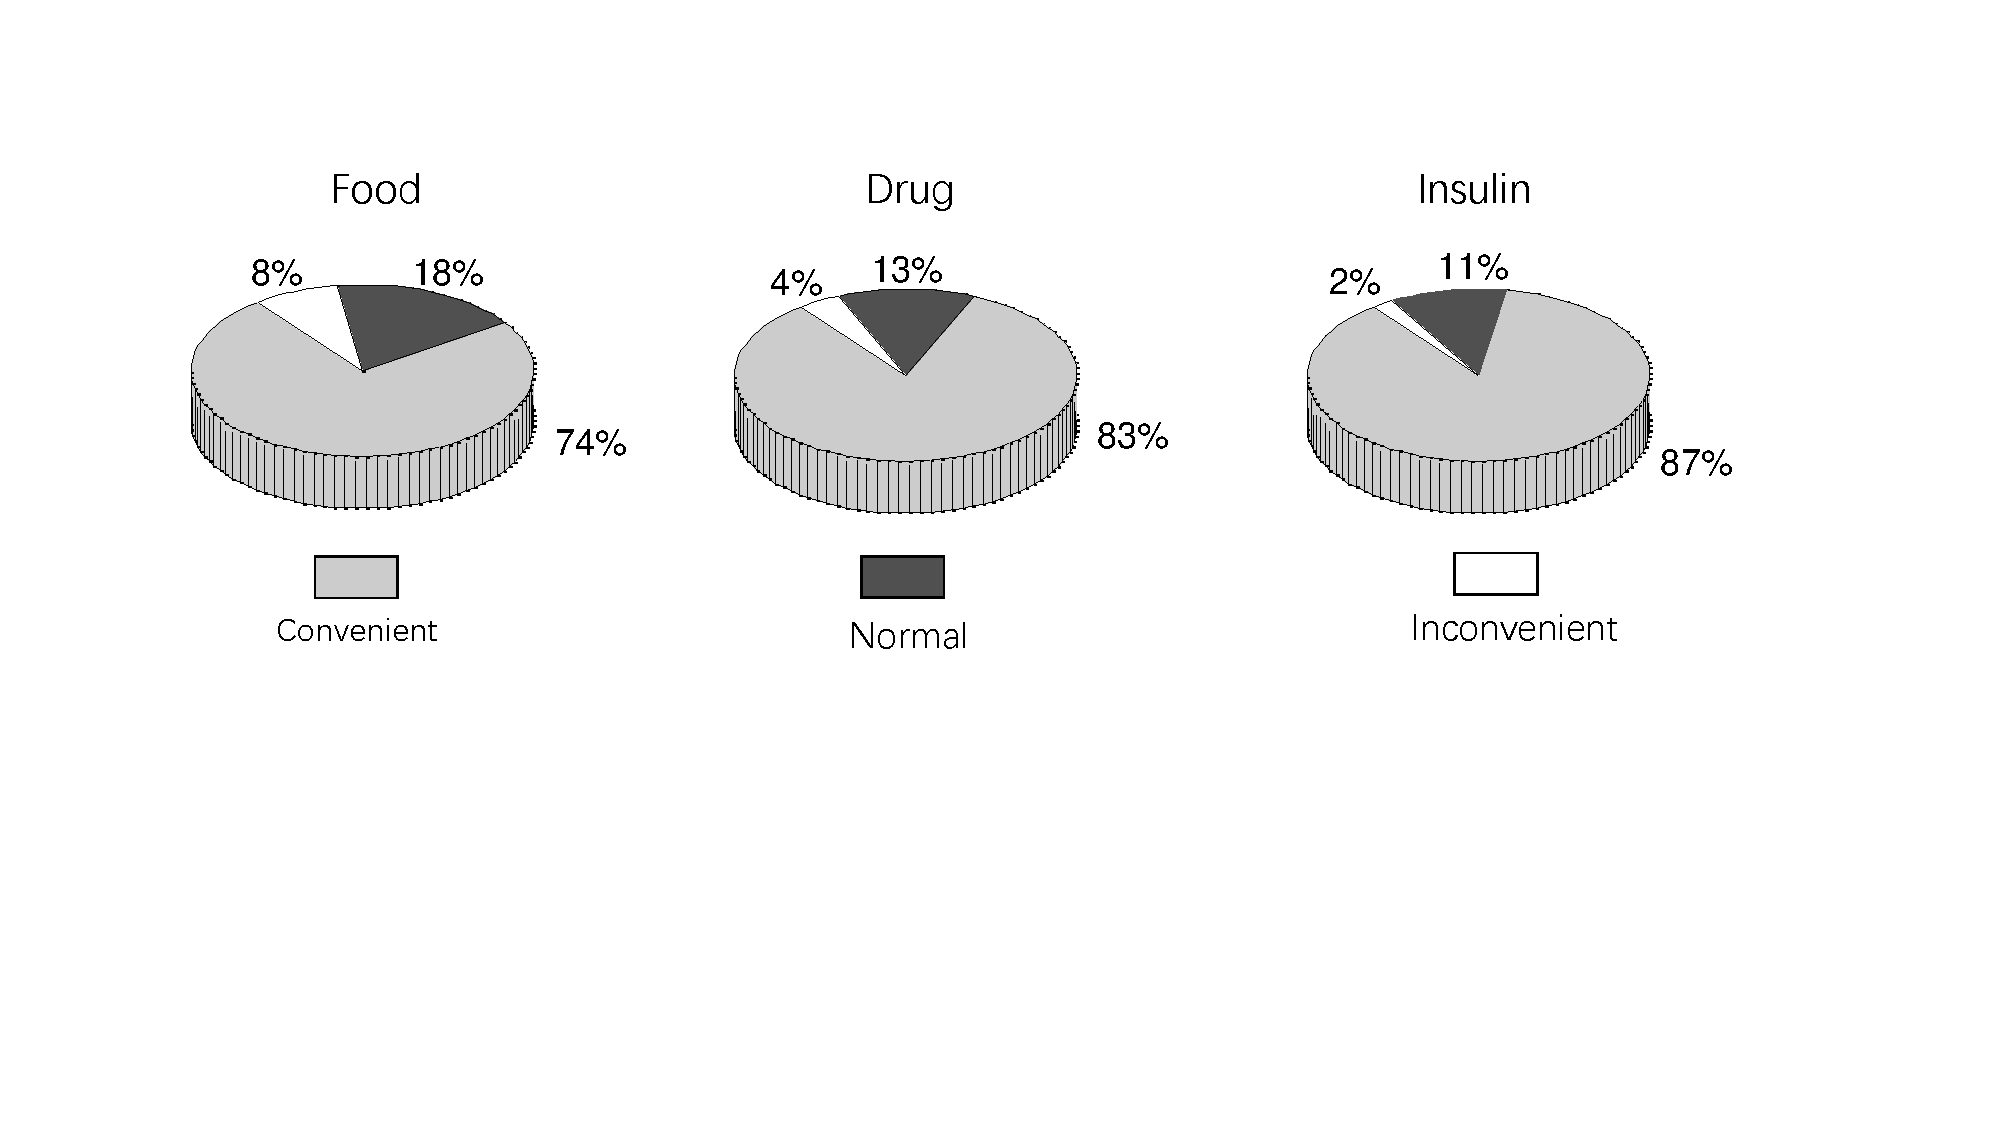
\includegraphics[width=0.8\columnwidth]{./img/user_cases.pdf}
  \caption{Distributions of  user comments on the operability of food, drug and insulin injection interfaces}
  \label{fig:user_cases}
\end{figure}


%\begin{figure}[h]
%  \centering
%  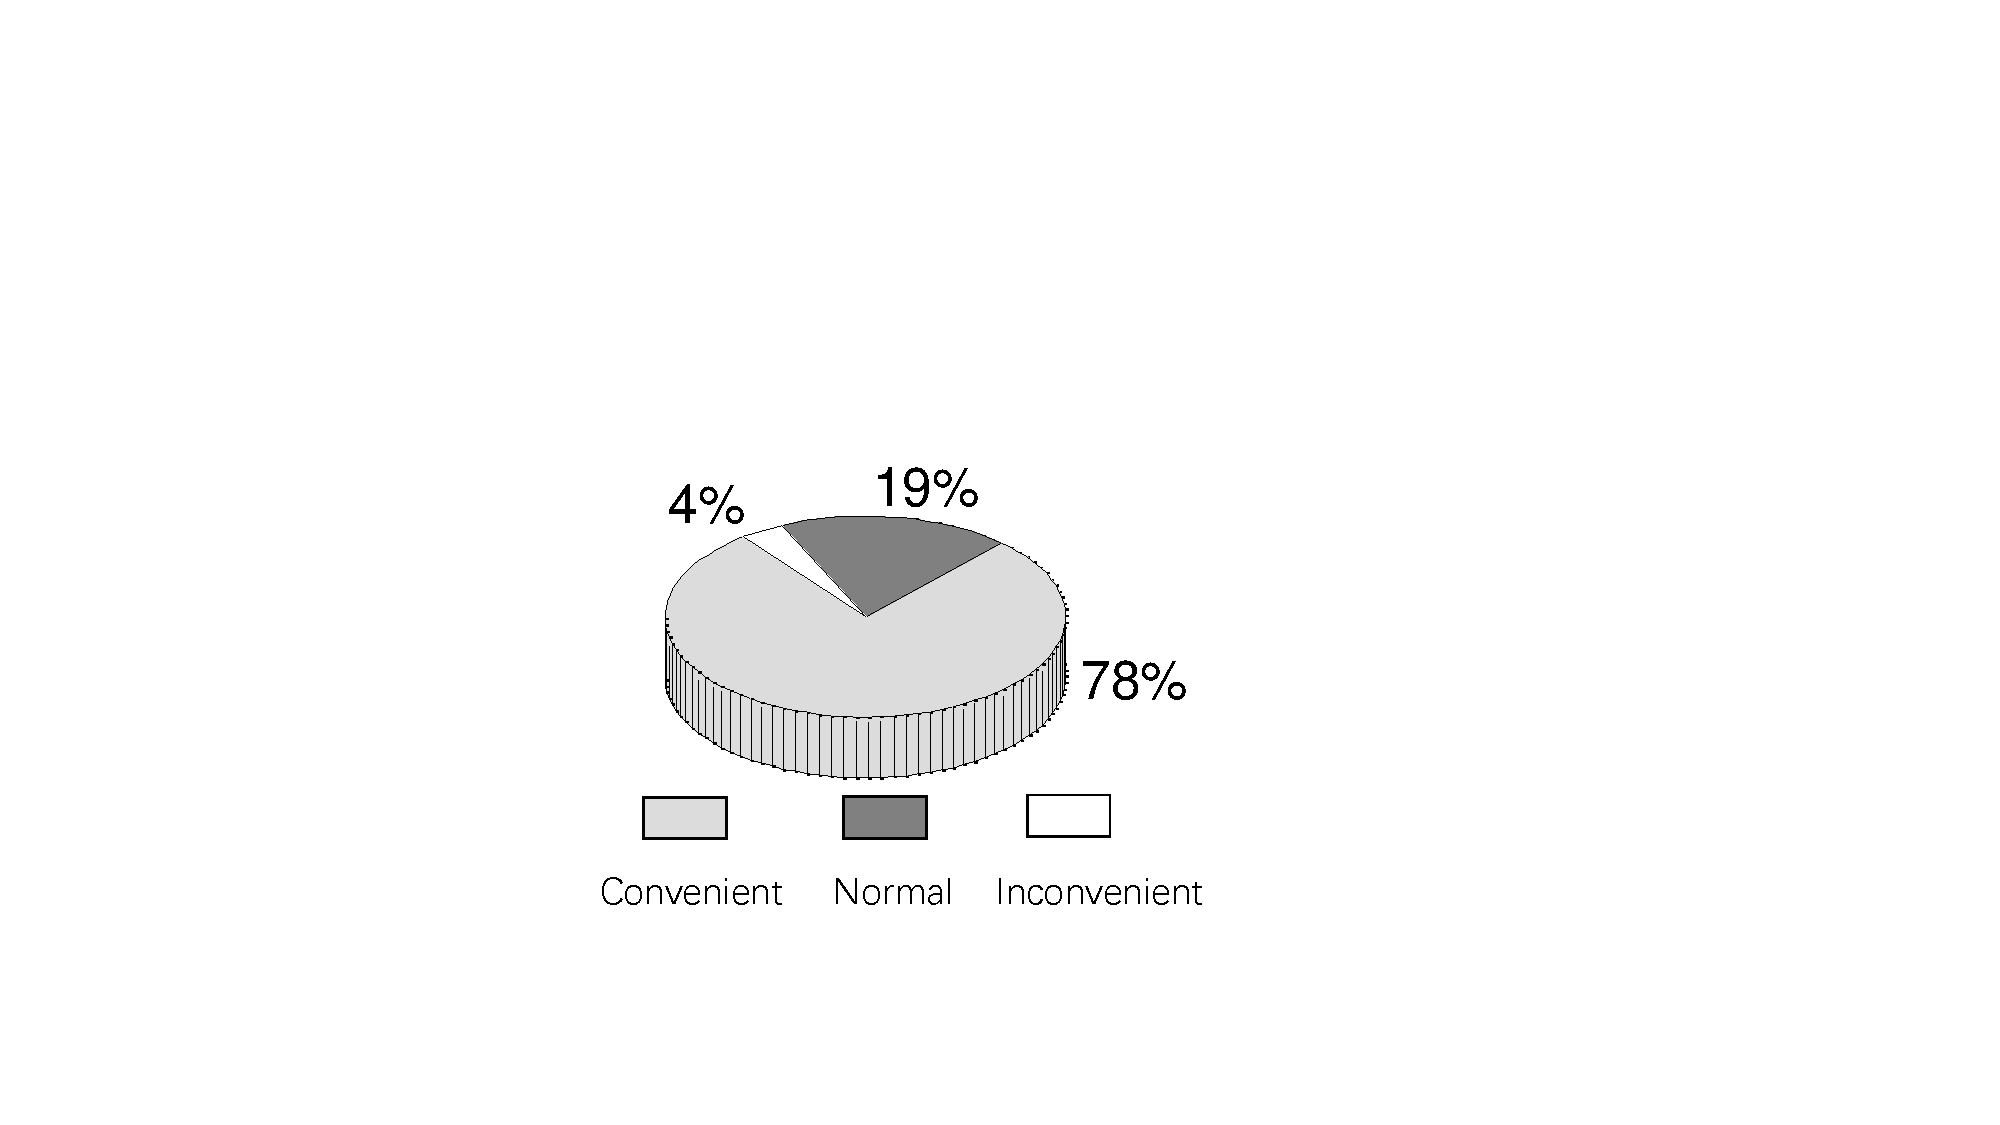
\includegraphics[width=0.3\columnwidth]{./img/usibility_levels.pdf}
%  \caption{Distributions of general comments of users}
%  \label{fig:usibility_levels}
%\end{figure}

In the questionnaire, we classify the system operability into three levels (\emph{i.e.}, \emph{Inconvenient}, \emph{Normal} and \emph{Convenient}).
Users are required to make comments on the operability of food input, drug input and insulin injection separately, as well as the final idea
on the whole system operability after their usage.
Fig.\ref{fig:user_cases} illustrates the  distributions of user comments on the operability of food, drug and insulin injection interfaces.
As for the food intake, 74\% users agree with the operability of \sysname is convenient, 18\% users hold the recoding process is normal, and the rest 8\% users maintain that \sysname is inconvenient. The comments of drug and insulin injection interfaces are slight better. The proportions of \emph{Convenient} at both cases are over 80\%, and those of \emph{Inconvenient} are less than 5\%. It is mainly due to the food intake is inconsistent and users need to input repeatedly during one day.

In final, the proportions of users who selected \emph{Inconvenient}, \emph{Normal} and \emph{Convenient} are 78\%, 18\% and 4\%. We select a representative comment of each level from users as follows:
\begin{itemize}
  \item  This app is easy to learn and quick to use. The database of foods, drugs and insulin is more extensive then I expected. I especially love the reminders that you can set now. Just a great app. [\emph{Convenient, type II user}]
  \item  I've some good experiences with this app. What I would like to see is a way to fill in the daily inputs by taking photo and speech. It would be more convenient to operate. Hoping to see these features in an upd
      ated version. [\emph{Normal, type I user}]
  \item The design of user interface still has room to improve. I expect more personalization in the app such as search hints or automate records based on my input history. If this comes true, my rating would go to 'Convenient'. [\emph{Inconvenient, health user}]
\end{itemize}

Based on our analysis, most comments from \emph{Normal} and \emph{Inconvenient} are about the manual records of drag, insulin and daily food. We also admit this limitation of human-computer interaction (HCI) on current prototype, and believe it can be well solved by many research works. Specifically, the suggestion mentioned by type I user can be coped with the current technologies such as computer vision \cite{bib:kawano2015foodcam} and speech recognition \cite{bib:hinton2012deep}.
The intelligent search hints and automatical item inputs suggested by type II user can also be learnt by the personal history data by recommendation algorithms \cite{bib:fu2000mining, bib:sarwar2001item}.
We are now working towards update our current version on these aspects.


\subsubsection{The instructions of \sysname}
We also ask whether users get instructions on the blood glucose control from \sysname. Each user first reports a general feedback from three
levels (\ie instructive, normal and non-instructive), and then gives comments in detail.
In general, 94\% participants are satisfied with the guidance of \sysname and report 'Instructive', 6\% users report 'Normal', and nobody gives
'non-instructive'.
We also listed two representative comments from two users (a 'Instructive' and a 'Normal'):

\begin{itemize}
  \item  \sysname guides me a lot on the blood glucose control, and literally changes my lifestyle. For instance, I always observe the blood glucose dynamics after meals, and figure out it rises significantly after I eat the noodle, bread and dumplings, but keeps a relative stable level after only eating meats and vegetables. I can also learn the impact of drugs on my blood glucose.
      It is not that the devices doing anything physically to change you life, but makes you more conscious of the way you are living your life. It presents a different perspective in front of you that allows you to make timely adjustment, and  help you avoid abnormal blood glucose level. I have recommended this products to six people who care about their glucose. Very  helpful, I like it.  [\emph{Instructive, type II user}]
  \item  I start to track my blood glucose. This app has made it easy but still has room to improve.
        It presents me a short-term impact of food intake.  However, I still care about how to maintain a long-term health status. Specifically,
        how to do exercise is health and how long we should do exercises to maintain a good blood glucose level. In this way, I can know how to prevent diabetes. [\emph{Normal, health user}]
\end{itemize}

In summary, \sysname gives suggestions on their meals, drugs and exercises \etc The users from \emph{'Normal'} level (most of whom are health) care about how to prevent diabetes or abnormal blood glucose cases. For this requirement, the personalized blood glucose dynamic records collected by \sysname can be synced to the experts communities, which can help the experts design a personalized precaution measurement.


\subsubsection{Energy overhead}
\begin{table}[t]
\centering
\caption{Profiles of smartphone }
\label{tab:smartphone_profiles}
\begin{tabular}{|l|l|l|l|l|l|}
\hline
\textbf{Type} & \textbf{CPU}    & \textbf{RAM} & \textbf{ROM} & \textbf{Power Capacity} & \textbf{Operation System} \\ \hline
Galaxy S6     & 8-cores 2.1 GHz & 3 GB         & 32 GB        & 2550m Ah                & Android 5.0               \\ \hline
HTC Desire A6 & 8-cores 1.7 GHz & 2 GB         & 16 GB        & 2600m Ah                & Android 5.0               \\ \hline
HUAWEI 4C     & 8-cores 1.2 GHz & 2 GB         & 8 GB         & 3100m Ah                & Android 4.4               \\ \hline
LenovoK80M    & 4-cores 1.8 GHz & 4 GB         & 64 GB        & 4000m Ah                & Android 4.4               \\ \hline
\end{tabular}
\end{table}






Let us recall the system workflow from the energy overhead perspective.  \sysname triggers the microphone, the accelerometer and the light sensor after the user choosing the sleeping mode, which is utilized to track the sleep quality of users. After the user waking up, \sysname shuts down the microphone and light sensor, only leaving an accelerometer to record the user's activities. Thus, \sysname conserves energy from two aspects: first, it keeps the sensors activated only around the right time; second, it adopts low-power sensors to reduce energy consumption.

To evaluate the battery conditions, \sysname are tested on four popular types of commercial phones (listed in Table \ref{tab:smartphone_profiles}) by volunteers. All of the smartphones are charged full of power (100\% percentage). Since \sysname is a service that could run in backstage, we lock the screen during this process and shut down all the applications except \sysname and a battery tracing application \cite{bib:PowerTutor}, which is installed in each smartphone to record the rest battery storage every two hours.  Fig.\ref{fig:battery_lifetime} illustrates the phone��s left battery as a function of execution time of \sysname.
\begin{figure}[h]
  \centering
  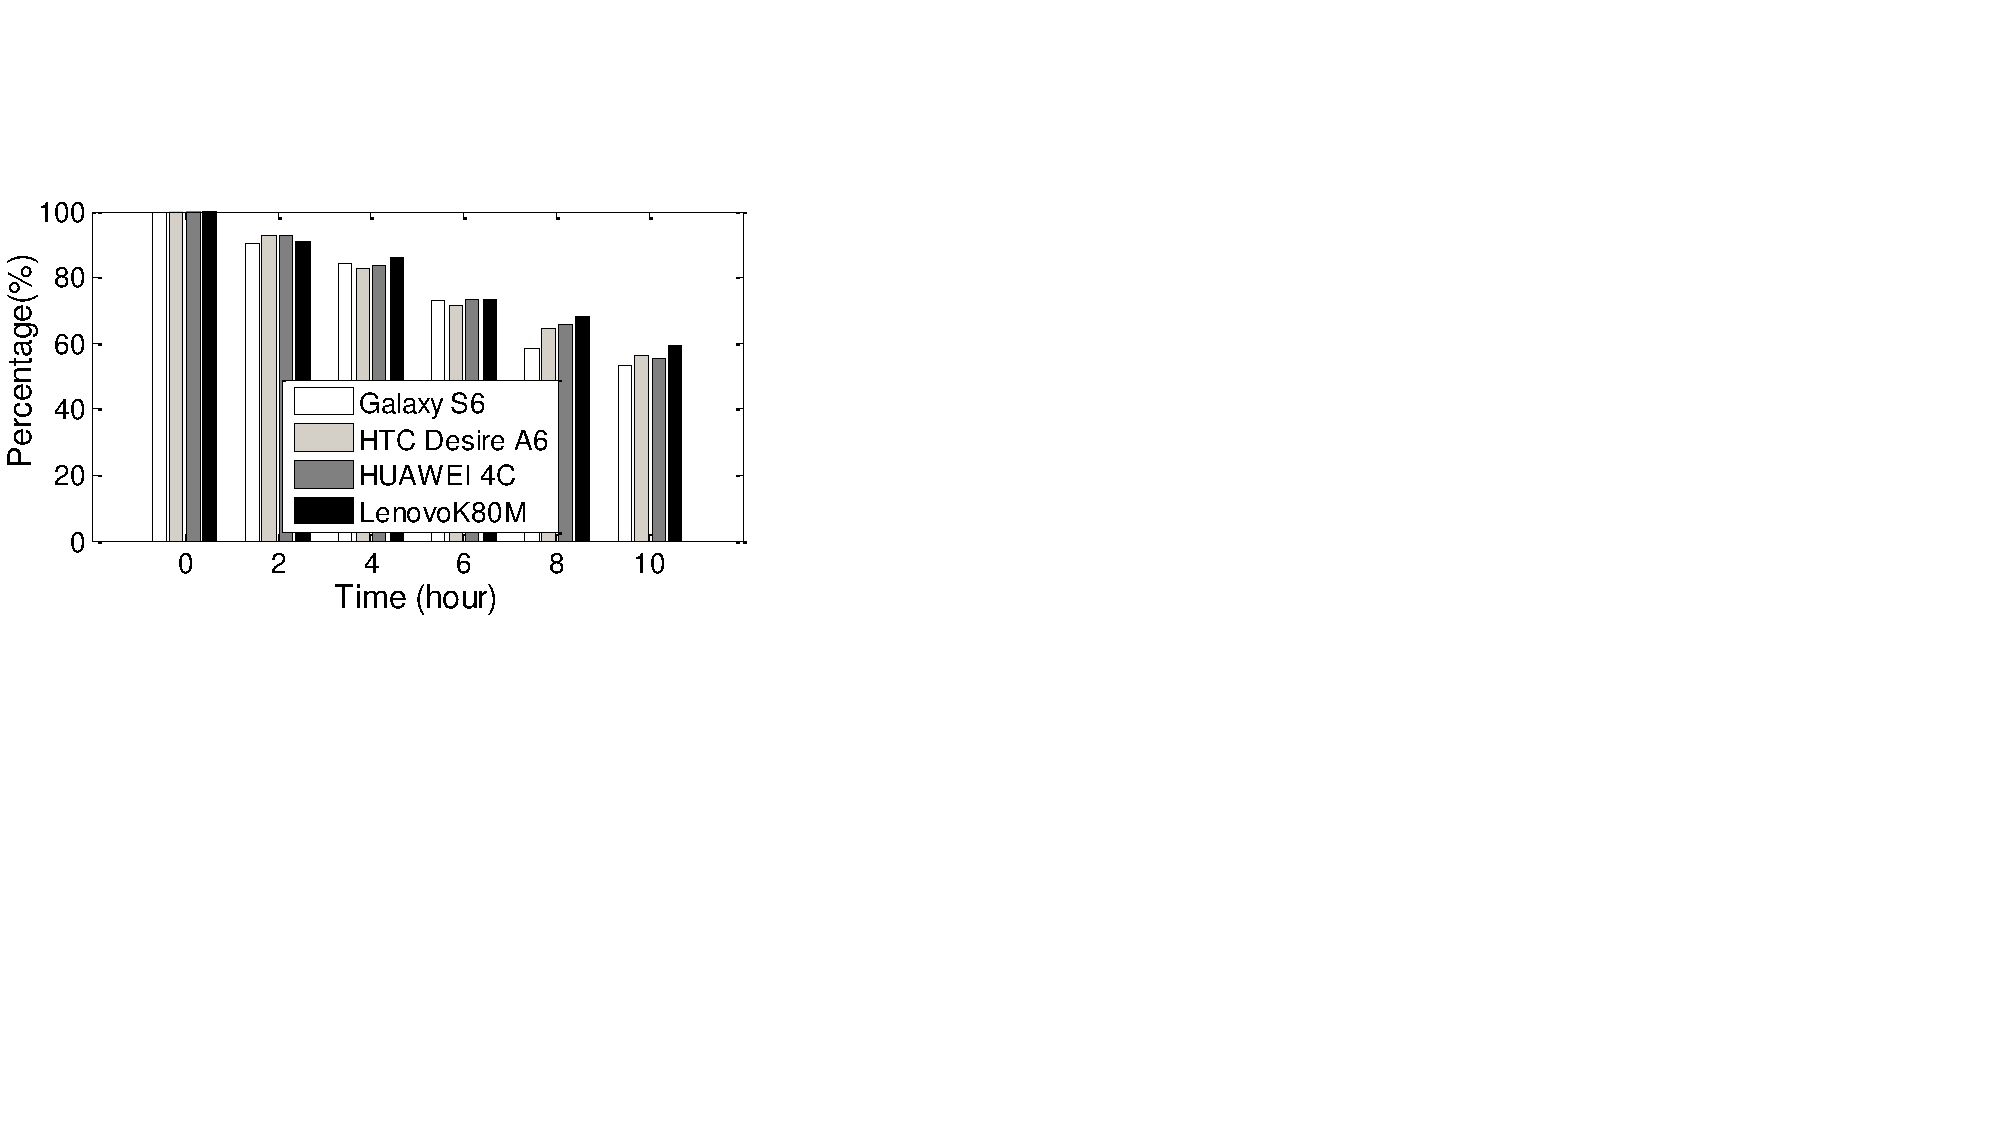
\includegraphics[width=0.5\columnwidth]{./img/battery_trace.pdf}
  \caption{Battery lifetime trace}
  \label{fig:battery_lifetime}
\end{figure}

As it indicates, the energy consumption presents a similar trend yet differs in amount for all of these four phones. Specifically, \sysname consumes energy around 10\% on average every two hours. With time passing by, the cumulative energy consumption increases
gradually, and finally ends up with about 50\% $\sim$ 60\%.

Fig.\ref{fig:battery_consumption} details the distribution of battery consumption in the experiments. \sysname only consumes less than 40\% of the whole energy, most power is costed by Android OS. That is to say, \sysname only costs less than 4\% battery every two hours, which is negligible and
affords for the daily use.

\begin{figure}[h]
  \centering
  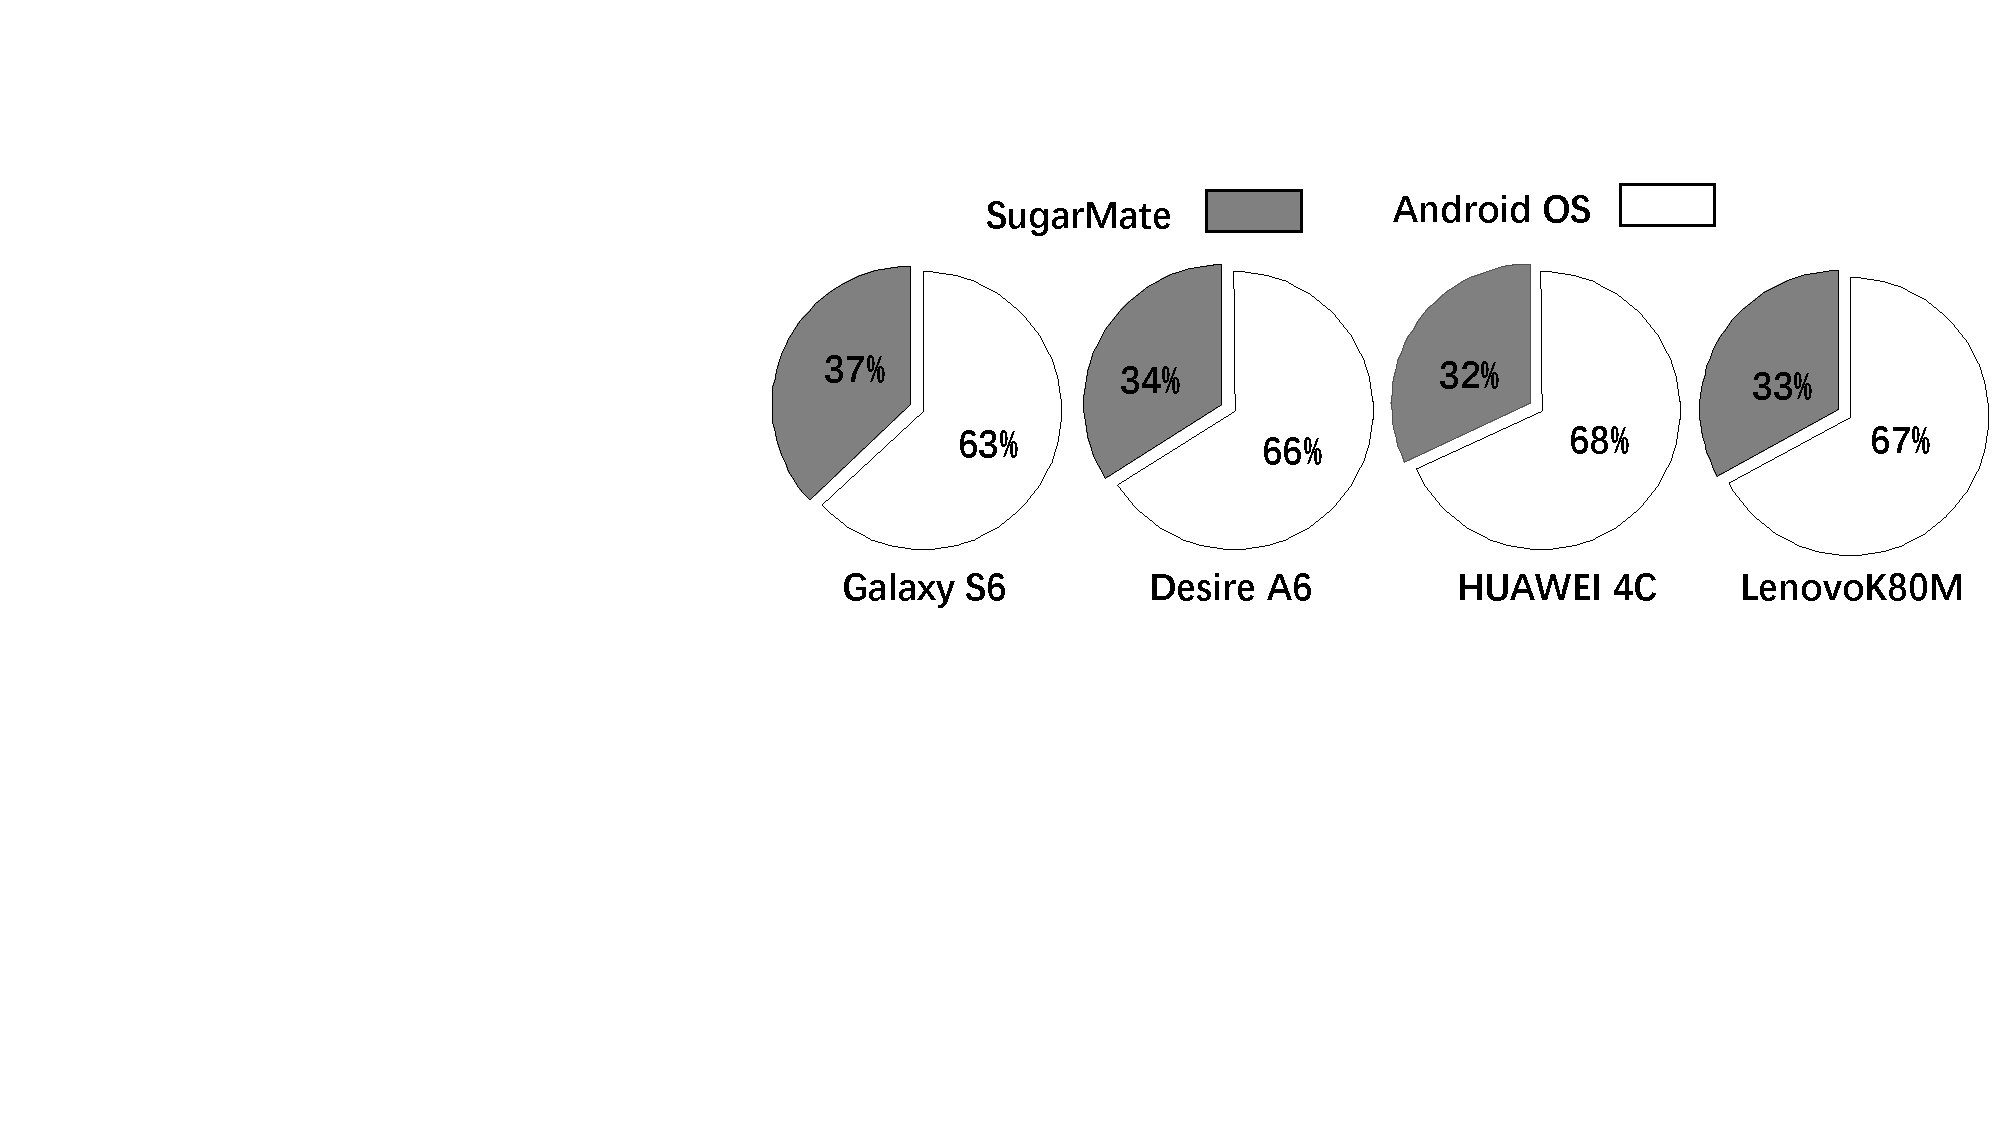
\includegraphics[width=0.7\columnwidth]{./img/energy_overhead.pdf}
  \caption{Battery consumption distribution}
  \label{fig:battery_consumption}
\end{figure}


